\documentclass{article}

% if you need to pass options to natbib, use, e.g.:
%     \PassOptionsToPackage{numbers, compress}{natbib}
% before loading neurips_2021

% ready for submission
\usepackage[preprint]{neurips_2021}

% to compile a preprint version, e.g., for submission to arXiv, add add the
% [preprint] option:
%     \usepackage[preprint]{neurips_2021}

% to compile a camera-ready version, add the [final] option, e.g.:
%     \usepackage[final]{neurips_2021}

% to avoid loading the natbib package, add option nonatbib:
%    \usepackage[nonatbib]{neurips_2021}

\usepackage[utf8]{inputenc} % allow utf-8 input
\usepackage[T1]{fontenc}    % use 8-bit T1 fonts
\usepackage{hyperref}       % hyperlinks
\usepackage{url}            % simple URL typesetting
\usepackage{booktabs}       % professional-quality tables
\usepackage{amsfonts}       % blackboard math symbols
\usepackage{nicefrac}       % compact symbols for 1/2, etc.
\usepackage{microtype}      % microtypography
\usepackage{xcolor}         % colors
\usepackage{graphicx}
\usepackage{subfig}

\title{Inflation in Chess Ratings}

% The \author macro works with any number of authors. There are two commands
% used to separate the names and addresses of multiple authors: \And and \AND.
%
% Using \And between authors leaves it to LaTeX to determine where to break the
% lines. Using \AND forces a line break at that point. So, if LaTeX puts 3 of 4
% authors names on the first line, and the last on the second line, try using
% \AND instead of \And before the third author name.

\author{%
  Voulgaris Sotirios\\
  Matrikelnummer 6013093\\
  \texttt{sotirios.voulgaris@student.uni-tuebingen.de} \\
}

\begin{document}

\maketitle

\begin{abstract}
The scope of the project\footnote{\url{https://github.com/Voulgaris-Sot/RatingInflationLichess}} is to examine if there are signs of inflation in the chess ratings of the Lichess webserver. We use the games that were analyzed by a chess engine in order to compute the Average CentiPawn Loss (ACPL) and investigate the effect that the side of the player and the rating has on ACPL and compare how ACPL has changed over time. The results indicate that there should be inflation across all ratings and time controls.
\end{abstract}

\section{Introduction}

Chess rating systems have always been an important part of online chess websites and are constantly a topic of debate. A chess rating is a measure of the relative skill of a player compared to other players in the same pool. Therefore the characteristics of a rating system change over time, depending on the skill level of the players and how they interact with each other. One interesting aspect of such rating systems is that they suffer from inflation or deflation, in other words the skill level of a rating level might change over time. Ratings are only affected by the result of the game and don’t take into account the game itself. On the contrary ACPL considers only how accurate the moves are according to a chess engine. We use this metric as a measure of chess skill in order to identify the relationship between the skill and rating.

\section{Background}

\subsection{Rating systems}

The first widely chess rating system was introduced in the 1950s by Arpad Elo, hence called “Elo system.” An improvement over the Elo system was proposed by Glicko in order to introduce a measure of the reliability of the rating. The Glicko-2 \cite{glicko2} calculates not only the rating of a player but also a rating deviation (RD) which can then be used to produce a confidence interval for the rating. The RD decreases after every game and will increase after a period of inactivity and is used for the calculation for the new ratings after every game. If a player has high RD then the system is not so certain about the rating and will try to push it faster to a value that is more representative of the skill of the player. 

In general, an Elo-like chess rating is only useful to compare players that play in the same pool and thus cannot be used to compare players across different pools - for example websites - or across a period of time. Rating systems are in a sense alive and its characteristics depend on the parameters of the systems which can change and its players. As a result, there are many practical problems that we have to take into account when we consider a rating system. For example, Glicko-2 tries to control for a players inactivity via the RD parameter and FIDE introduced inflation mechanism to combat the fact that in a pure Elo system the ratings gradually deflate. Rating deflation occurs when the playing strength of players of a specific rating bracket is increasing, while the reverse is true is the case of inflation.

\subsection{Chess Engines and Machine Evaluation}
Chess is famously referred as the ‘drosophila’ of artificial intelligence (AI) \cite{drosophilia} during the early days of AI research. The reason is simple: chess is a game with perfect knowledge and simple rules while at the same time being very hard to master for most humans. Chess represented the extend of the human intelligence and was ideal for the demonstration of AI advancements. The goal was to construct a computer program – a chess engine – which was able to play and win against the best human chess players, a dream that was finally fulfilled by the Deep Blue system against the reigning world chess champion Garry Kasparov in 1997. This victory was considered a huge milestone in the history of AI but since then chess engines have only become better and better. Nowadays, the question is not if but how much stronger the engines are compared to humans.

At the highest level of abstraction, chess engines take as input a chess position and generate a list of moves that are considered the strongest. The ranking of the moves is according to an evaluation that the engine assigns to each position. In other words, the engine can act us an oracle that can give a pretty good estimation of the true evaluation of a chess position. However, the domination of the chess engines does not mean that the interest in chess have decreased. On the contrary, the chess engine have helped us to better understand the game and make it more accessible to beginners, because it is now easier than ever to check how well you are doing according to the evaluation of the chess engine. 

\subsection{Average centipawn loss}
The Elo-like chess rating systems take into account only on the result of the game to estimate the playing strength of a chess player. However in \cite{icr,Alliot,Guid} they try to estimate the true playing strength by the quality of their moves during the game. These methods use the evaluations of a computer engine and try to compare the actual moves played in the games against the moves that were proposed as best from a chess engine. A common and straightforward metric that can be used is the Average CentiPawn Loss (ACPL). The centipawn loss is the difference in the evaluation of the chess board before and after a player made a move. This difference is then averaged over all the moves and we arrive at a single number for each player (ACPL) with symbolizes how close that player followed the best moves as proposed by the engine.
The advantage of this approach for is that we don’t compare players to each other and their respective results but only compare against the evaluations of a chess engine. We thus have another way to look at a players strength that is independent of its pool and this can help us to analyze the Elo-like rating distribution pools and identify common problems they have like inflation.


\section{Methodology}

In this project we focus on two main questions:

\begin{itemize}

\item Is ACPL a reliable metric of players strength?
\item Can ACPL be used as an indicator of rating inflation?

\end{itemize}

For our analysis we used the Lichess database \footnote{\url{https://database.lichess.org/}}, which consists of all standard rated games since 2013 that were played on the open source Lichess Internet chess server\footnote{\url{https://lichess.org/}}. Lichess uses the Glicko-2 rating system with a starting rating of 1500 and there are different ratings for each time control control. The time controls in order of decreasing popularity are blitz, rapid, bullet and classical. Blitz games last 3 to 8 minutes, bullet games less than 3 minutes, rapid between 8 and 25 and classic games last more than 25 minutes. In order to compute the ACPL we need access to the evaluation from a chess engine and around 6\% of the games were analyzed per the request of the users from Lichess. The evaluations are produced via the Stockfish game engine \footnote{\url{https://stockfishchess.org/}} and for games over 100 moves long the evaluations stop at the 100 move. The Lichess database contains so far 2,911,084,203 games and in order to make the project feasible we focused on a subset of the games. For the first part we used the analyzed games from 2019 ($\sim$26,000,000 games) and for the second part we used the games from the November of each year in the period 2014-2021 ($\sim$18,000,000 games).

For the ACPL calculation we replicated the algorithm that Lichess uses. The initial evaluation before white makes the first move is 15 centipawns and the evaluations are capped to 1000 centipawns because it is considered enough of a winning advantage and anything over that is practically winning. We then compute the centipawn loss for each player and average to obtain the ACPL. Theoretically, the centipawn loss after each move cannot be positive as you cannot make the position better but practically this can happen because of limited precision of the engine in wcich case we set the loss to 0. 
Finally, in order to avoid outliers and have a more clear view of the results we restricted our analysis on players that have a rating between 800 to 2750 (~96\% of the players) and we filtered out games that were under 10 moves or had ACPL over 500.

\section{Results}

Before considering the relation between rating and ACPL, we have to examine the effect that the side of player (white or black) and time control have on ACPL.  As illustrated in Figure 1 we can see that the distribution between black and white players is very similar with black having a slightly heavier tail as indicated by the average ACPL in Table 1. As for the time controls, the faster the game the higher the average ACPL because players don’t care or don’t have the time to find the absolutely best moves.

\begin{table}[h]
\caption{Average ACPL}
\centering
\begin{tabular}{lrrr}

\toprule
{} &  black ACPL &  white ACPL &     Count \\
Time Control &             &             &           \\
\midrule
Blitz        &       75.34 &       72.88 &  11233853 \\
Bullter      &       84.01 &       82.12 &   5551209 \\
Classical    &       74.88 &       72.39 &   3269814 \\
Rapid        &       74.11 &       71.76 &   5870412 \\
\bottomrule
\end{tabular}
\end{table}

\begin{figure}
  \centering
%  \fbox{\rule[-.5cm]{0cm}{4cm} \rule[-.5cm]{4cm}{0cm}}
  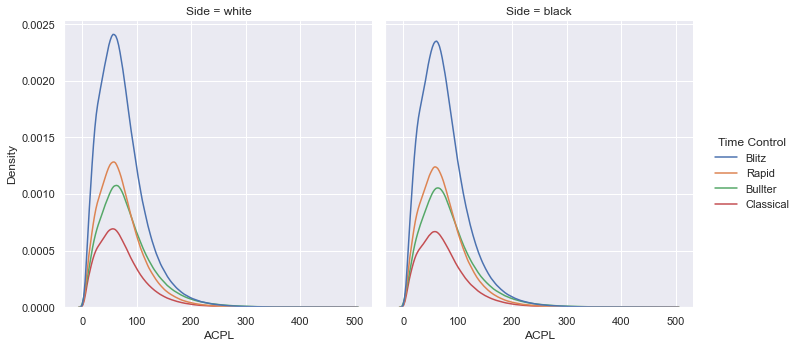
\includegraphics[width=\linewidth]{images/Fig-1.png}
  \caption{Distribution of ACPL per side and time control}
\end{figure}

Because the overall shape of the distributions for the different time controls are similar with the only difference being how quickly the tail drops to zero, we will now focus only on the blitz time control because it is by far the most popular. Figure 2 presents the distribution of the white and black side for different rating levels.
It is interesting to observe that the slight difference between the black and side that we observed before is consistent across all levels and white has always a smaller mean ACPL. However the gap is more significant is the smaller rating levels, which might indicate that lower rated player play more accurately when they are on the white side. Moreover, we can see that the higher the rating, the smaller the mean ACPL and as for the actual distributions in the case of the lower rated players they are more smooth and the mode is much closer to the mean compared to the high rated players, in which case most of the mass is closer to the first quartile. Overall, there is a clear relationship between ACPL and rating, with higher rated players having significantly lower ACPL on average.
 
\begin{figure}
  \centering
%  \fbox{\rule[-.5cm]{0cm}{4cm} \rule[-.5cm]{4cm}{0cm}}
  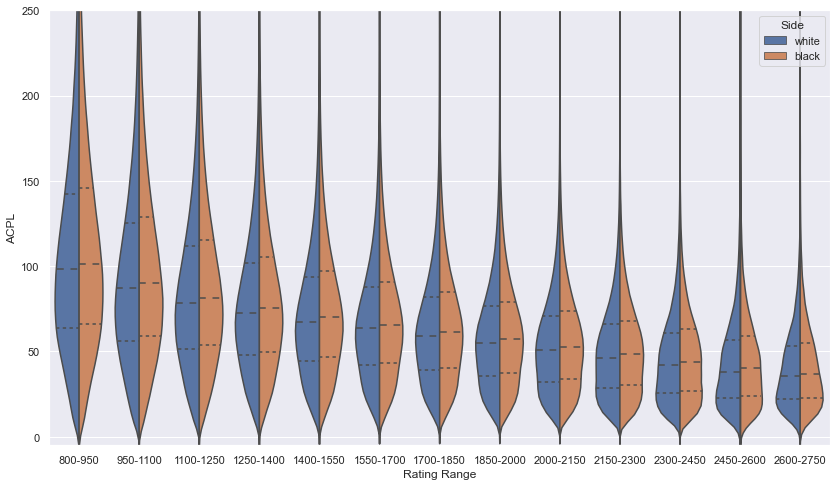
\includegraphics[width=0.9\linewidth, keepaspectratio]{images/Fig-2.png}
  \caption{Distribution of ACPL in blitz for different rating levels}
\end{figure}
\begin{figure}
  \centering
%  \fbox{\rule[-.5cm]{0cm}{4cm} \rule[-.5cm]{4cm}{0cm}}
  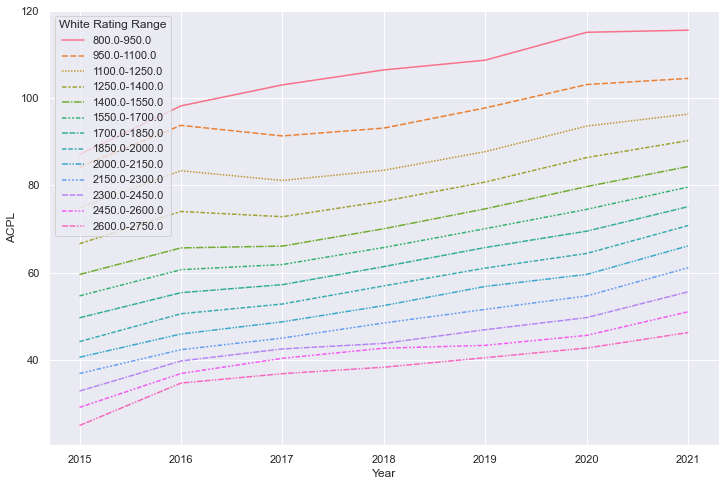
\includegraphics[width=\linewidth]{images/Fig-3.png}
  \caption{Average ACPL for the white side and blitz time control}
\end{figure}

Now that we have established that there is a relationship between the rating level and ACPL he want to know if the level of accuracy changes over time, in other words if there is any rating inflation. Figure 3 illustrates how the mean ACPL for the white side and for the blitz time control changes over time for each rating range. Similar results can be obtained for the black side and for different time controls. We observe that in most cases the mean ACPL grows each year. This implies that if accept the ACPL as an acceptable measure of chess strength, then there is rating inflation which grows stronger by the year. A player with average rating 1800 plays much less accurate than someone with the same rating a few years ago. 

\section{Limitations}
Our analysis does not come without limitations, on the contrary there are many things we should pay attention to when consider the results. First of all, ACPL depends on the chess engine we use and how strong it is. Every year the chess engine are becoming stronger and stronger and their evaluations become more accurate. In our data, we have evaluations from many different engines depending on which version of the Stockfish engine Lichess used at the time. Furthermore, we didn’t have control on what games where analyzed. The games where annotated with evaluations only after the request of the players and it is possible that there is a bias toward which games are analyzed and which are left with no evaluations. Finally and perhaps most importantly, it is not clear how much we can depend on the ACPL as a measure of chess strength. It is clear that if we look at a single game, the ACPL is not a good indicator because a player can make a lot of bad moves and still win because in the end it matters who makes the last mistake or who is slower and loses on time. However, we believe that if we look at the total distribution of the ACPL then we can make some interesting insights as we tried to show on our analysis.

Consider donating to Lichess for their awesome open source work they are doing.

\bibliographystyle{plain}
\bibliography{report}

\end{document}
